\graphicspath{{chapters/gradient_descent/}}


\chapter{Efficient Algorithms for the CCA Family: Unconstrained Losses with Unbiased Gradients}\label{chap:gradient_descent}
\epigraph{It seems easier to train a bi-directional LSTM with attention than to compute the SVD of a large matrix.\cite{gemp}}{Chris Ré}
\minitoc
% chktex-file 44
% chktex-file 3
\section*{Preface}
The content of this chapter is based on a series of papers~\citep{chapman2022generalized, chapman2023efficient} as well as a NeurIPS workshop paper~\citep{chapman2023neurips}.
I am grateful to my co-authors Lennie Wells and Ana Lawry Aguila for their contributions to this work.
In particular, Lennie's mathematical expertise improved the theoretical grounding of the idea greatly and Ana's access to the UK Biobank dataset enabled the application of our methods to a real-world biomedical dataset.
In this thesis I include much of the work from these papers, but I exclude many of Lennie's extensive proofs where I can make no claim to have contributed beyond proofreading.

\section{Introduction}

T


\section{Background: Efficient CCA}\label{sec:background-unified}

\subsubsection{Challenges in Solving Generalized Eigenvalue Problems}

The GEP is often represented as \( Ax = \lambda Bx \), where \( A \) and \( B \) are matrices. To generalize the dimensions of these matrices, let's denote them as \( m \times m \). This dimension \( m \) can vary based on the specific method in use. For instance, in Principal Component Analysis (PCA), represented as \acrshort{pca}, \( m \) would be equal to \( p \) since \( A \) and \( B \) are \( p \times p \) matrices. In methods like Partial Least Squares (PLS) and Canonical Correlation Analysis (CCA), represented as \acrshort{pls} and \acrshort{cca} respectively, \( m \) would be \( p+q \), as \( A \) and \( B \) in these cases are \( (p+q) \times (p+q) \).


% Table summarizing the definitions of A and B for various methods
\begin{table}[h]
    \centering
    \begin{tabular}{|c|c|c|c|c|}
        \hline
        Method         & \( A \)           & \( B \)   & \( x \)        & Dimensions       \\
        \hline
        \acrshort{pca} & \( \Sigma_{11} \) & \( I \)   & \( u\sps{1} \) & \( p \times p \) \\
        \hline
        LDA            & \( S_B \)         & \( S_W \) & \( u\sps{1} \) & \( p \times p \) \\
        \hline
        \acrshort{cca} & \( \begin{pmatrix}
                                \Sigma_{11} & \Sigma_{12} \\ \Sigma_{21} & \Sigma_{22}
        \end{pmatrix} \) & \( \begin{pmatrix}
                                  \Sigma_{11} & 0 \\ 0 & \Sigma_{22}
        \end{pmatrix} \) & \( \begin{pmatrix}
                                  u\sps{1} \\ u\sps{2}
        \end{pmatrix} \) & \( (p+q) \times (p+q) \) \\
        \hline
        \acrshort{pls} & \( \begin{pmatrix}
                                0 & \Sigma_{12} \\ \Sigma_{21} & 0
        \end{pmatrix} \) & \( I \) & \( \begin{pmatrix}
                                            u\sps{1} \\ u\sps{2}
        \end{pmatrix} \) & \( (p+q) \times (p+q) \) \\
        \hline
    \end{tabular}
    \caption{Definitions and dimensions of \( A \)and \( B \)for different subspace learning methods.}
    \label{tab:subspace}
\end{table}

To solve the GEP, one common technique is to transform it into a standard eigenvalue problem \( B^{-\frac{1}{2}} A B^{-\frac{1}{2}} y = \lambda y \), followed by eigendecomposition. However, this approach has computational complexity \( O(m^3) \) and may suffer from numerical instability.

\subsubsection{\acrshort{pca}-CCA}

One way to reduce the complexity of solving GEPs is to use the \acrshort{pca}-CCA method, which first applies \acrshort{pca} to the data and then solves the GEP in the reduced space.
An important advantage of using \acrshort{pca}-CCA is computational efficiency, especially for high-dimensional data.
The overall complexity of \acrshort{pca}-CCA involves two main steps.
First, applying PCA has a complexity of \( O(\max(p^3, q^3)) \), dominated by the larger of the two matrices.
Second, solving the generalized eigenvalue problem in the reduced space with \( K \) components in each view leads to a complexity of \( O((2K)^3) \).
Thus, the overall complexity of \acrshort{pca}-CCA is \( O(\max(p^3, q^3) + (2K)^3) \), which is significantly lower than the complexity of solving the GEP directly.
Since CCA, ridge CCA, and PLS can all be solved in the principal component space, \acrshort{pca}-CCA can be used to compute solutions efficiently \textit{even if we keep all the principal components}.
Most obviously, this is the case when the number of samples \( n \) is smaller than either of the number of features \( p \) or \( q \), i.e. \( n < p \) or \( n < q \).
In this case the maximum number of principal components is \( K=n \), and the complexity of \acrshort{pca}-CCA is thus \( O(n^3) \), which is significantly lower than the complexity of solving the GEP directly.
This approach has been employed to great effect in neuroimaging but suprisingly is not used even in the scikit-learn implementation of \acrshort{cca} \citep{pedregosa2011scikit}.
Nonetheless, for the large sample sizes (desirable for machine learning frameworks as well as statistical power), the complexity of even \acrshort{pca}-CCA can render the problems nearly intractable.

Kernel \acrshort{cca} (\acrshort{kcca}) also offers computational efficiency for high-dimensional data (\(p>n\)) as its complexity scales with the number of samples \(n\), not the number of features \(p\).
It casts the CCA optimisation as a dual problem:

\begin{align}
    & \alpha_{\text{opt}}=\underset{\alpha_{\text{opt}}}{\mathrm{argmax}}\{ \alpha\sps{1}K\spsT{1}K\sps{2}\alpha\sps{2}  \} \\
    & \text{subject to:} \notag                                                                                            \\
    & \alpha\sps{1}K\spsT{1}K\sps{1}\alpha\sps{1}=1 \notag                                                                  \\
    & \alpha\sps{2}K\spsT{2}K\sps{2}\alpha\sps{2}=1 \notag
\end{align}

Where \(\alpha\sps{1}=\)

The kernel function in KCCA can be computed iteratively on pairwise comparisons of samples, allowing for memory efficiency by not requiring the entire dataset to be loaded into RAM.
This iterative approach uses slow hard drive memory access instead of RAM, making KCCA RAM memory-efficient but slower.
However, a significant drawback of KCCA is the need for access to all training data at test time, which raises concerns about efficiency and scalability.


\subsection{Stochastic PLS and CCA}


To the best of our knowledge, the state-of-the-art in Stochastic PLS and CCA are the subspace Generalized Hebbian Algorithm (\textbf{SGHA}) of \cite{chen2019constrained} and \textbf{$\gamma$-EigenGame} from \cite{gemp20,gemp2021}. Specifically, SGHA utilizes a Lagrange multiplier heuristic along with saddle-point analysis, albeit with limited convergence guarantees. EigenGame focuses on top-k subspace learning but introduces an adaptive whitening matrix in the stochastic setting with an additional hyperparameter. Both methods set the benchmarks we aim to compare against in the subsequent experimental section. Like our method, both can tackle other symmetric Generalized Eigenvalue Problems in principle.


\section{Novel Objectives and Algorithms}\label{sec:contributions}
\subsection{Unconstrained objective for GEPs}\label{sec:gep-ey-formulation}
First, we present proposition \ref{prop:EY-charac}, a formulation of the top-$K$ subspace of GEP problems, which follows by applying the Eckhart--Young--Minsky inequality \citep{stewart_matrix_1990} to the eigen-decomposition of $B^\mhalf A B^\mhalf$. However, making this rigorous requires some technical care which we defer to the proof in supplement \ref{supp:proofs}.

\begin{restatable}[Eckhart--Young inspired objective for GEPs]{proposition}{EYcharac}
    \label{prop:EY-charac}
    The top-$K$ subspace of the GEP $(A,B)$ can be characterized by minimizing the following objective over $U \in \R^{D \times K}$:
    \begin{align}\label{eq:EY-charac}
    \LEYGEP(U) \defeq \tr \left( - 2\,U^T A U + \left(U^T B U\right) \left(U^T B U\right) \right)
    \end{align}
    Moreover, the minimum value is precisely $- \sum_{k=1}^K \lambda_k^2$, where $(\lambda_k)$ are the generalized eigenvalues.
\end{restatable}

This objective also has appealing geometrical properties.
It is closely related to a wide class of unconstrained objectives for PCA and matrix completion which have no spurious local optima \citep{ge_no_2017}, i.e. all local optima are in fact global optima.
This implies that certain local search algorithms, such as stochastic gradient descent, should indeed converge to a global optimum.

\begin{restatable}{proposition}{NoSpuriousLocalMinima}[No spurious local minima]\label{prop:no-spurious}
The objective $\LEYGEP$ has no spurious local minima.
That is, any matrix $\bar{U}$ that is a local minimum of $\LEYGEP$ must in fact be a global minimum.
        %of the form described in \cref{prop:EY-charac}
\end{restatable}

It is also possible to make this argument quantitative by proving a version of the strict saddle property from \cite{ge_no_2017,ge2015escaping}; we state an informal version here and give full details in \cref{supp:tractable-optimization}.

\begin{corollary}[Informal: Polynomial-time Optimization]
    Under certain conditions on the eigenvalues and generalized eigenvalues of $(A,B)$, one can make quantitative the claim that:
    any $U_K \in \R^{D \times K}$ is either close to a global optimum, has a large gradient $\nabla \LEYGEP$, or has Hessian $\nabla^2 \LEYGEP$ with a large negative eigenvalue.

    Therefore, for appropriate step-size sequences, certain local search algorithms, such as sufficiently noisy SGD, will converge in polynomial time with high probability.
        % still need to sort out - polynomial in what exactly!
\end{corollary}

\subsection{Corresponding Objectives for the CCA family}
For the case of linear CCA we have $U^T A U = \sum_{i \neq j} \Cov(Z\sps{i}, Z\sps{j}), U^T B U = \sum_{i} \Var(Z\sps{i})$.
To help us extend this to the general case of nonlinear transformations, \cref{eq:general-form-of-representations}, we define the analogous matrices of total between-view covariance and total within-view variance
\begin{align}\label{eq:def-C-V-matrices}
\vphantom{\bigl(\bigr)} % increase vertical space
C(\theta) = \sum_{i \neq j} \Cov(Z\sps{i}, Z\sps{j}), \quad
V(\theta) = \sum_{i} \Var(Z\sps{i})
\end{align}
In the case of linear transformations, \cref{eq:cca-linear-function-def}, it makes sense to add a ridge penalty so we can define
\begin{align}\label{eq:v-alpha-ridge-definition}
V_\alpha(\theta) = \sum_i \alpha_i {U\spsT{i}} U\sps{i} +  (1 - \alpha_i) \Var(Z\sps{i})
\end{align}
This immediately leads to following unconstrained objective for the CCA-family of problems.
\begin{definition}[Family of EY Objectives]
    Learn representations $Z\sps{i} = f\sps{i}( X\sps{i}; \theta\sps{i})$ minimizing
    \begin{align}\label{eq:EY-loss-def-C-V}
    \LEY(\theta) = - 2 \tr C(\theta) + \norm{V_\alpha(\theta)}_F^2
    \end{align}
\end{definition}

\textbf{Unbiased estimates:}
since empirical covariance matrices are unbiased, we can construct unbiased estimates to $C, V$ from a batch of transformed variables $\Z$.
\begin{align}\label{eq:def-C-V-matrices-empirical}
\hat{C}(\theta)[\Z] = \sum_{i \neq j} \empCov(\Z\sps{i}, \Z\sps{j}), \quad
\hat{V}(\theta)[\Z] = \sum_{i} \empVar(\Z\sps{i})
\end{align}
In the linear case we can construct $\hat{V}_\alpha(\theta)[\Z]$ analogously by plugging sample covariances into \cref{eq:v-alpha-ridge-definition}.
Then if $\Z, \Z'$ are two independent batches of transformed variables, the batch loss
\begin{align}\label{eq:empirical-EY-loss-estimate-def}
\empLEY[\Z, \Z'] \defeq - 2 \tr \hat{C}[\Z] + \langle \hat{V}_\alpha[\Z], \hat{V}_\alpha[\Z'] \rangle_F
\end{align}
gives an unbiased estimate of $\LEY(\theta)$.%\footnote{Where again $\alpha > 0$ only makes sense in the linear case, and otherwise we may omit the $\alpha$s}
This loss is a differentiable function of $\Z, \Z'$ and so also of $\theta$.

\textbf{Simple algorithms:}
We first define a very general algorithm using these estimates in Algorithm \ref{alg:general}.
In the next section we apply this algorithm to multi-view stochastic CCA and PLS.

\begin{algorithm}
    \caption{GEP-EY: General algorithm for learning correlated representations}
    \label{alg:general}
    \begin{algorithmic}
        \STATE {\bfseries Input:} data stream of mini-batches $(\X(b))_{b=1}^\infty$ where each consists of $M$ samples from the original dataset. Learning rate $(\eta_t)_t$. Number of time steps $T$. Class of functions $f(\cdot; \theta)$ whose outputs are differentiable with respect to $\theta$.
        \STATE {\bfseries Initialize:} $\hat{\theta}$ with suitably random entries
        \FOR{$t=1$ {\bfseries to} $T$}
        \STATE Obtain two independent mini-batches \( \X(b), \X(b') \) by sampling \( b, b' \) independently
        \STATE Compute batches of transformed variables $\Z(b) = f(\X(b); \theta), \Z(b') = f(\X(b'); \theta)$
        %\STATE Construct unbiased estimates $C(\theta)[\Z], \hat{V}(\theta)[\Z], \hat{V}(\theta)[\Z']$ \COMMENT{As defined in \cref{eq:def-C-V-matrices-empirical}}
        \STATE Estimate loss $\empLEY(\theta)$ using \cref{eq:empirical-EY-loss-estimate-def}
        \STATE Obtain gradients by back-propagation and step with your favourite optimizer.
        \ENDFOR
    \end{algorithmic}
\end{algorithm}

\subsection{Applications to (multi-view) stochastic CCA and PLS}
\begin{lemma}[Objective recovers GEP formulation of linear (multi-view) CCA]
    When the $f\sps{i}$ are linear, as in \cref{eq:cca-linear-function-def}, the population loss from \cref{eq:EY-loss-def-C-V} recovers MCCA as defined in \cref{sec:CCA-family}. %Moreover, the minimal loss value is precisely $-\norm{\MCCA_K(X)}$
\end{lemma}
\begin{proof}
    By construction, for linear MCCA we have $C = U^T A U,\, V_\alpha=U^T B_\alpha U$, where $(A, B_\alpha)$ define the GEP for MCCA introduced in \cref{eq:gep-most-general-formulation}.
    So $\LEY(U) = \LEYGEP(U)$ and by \cref{prop:EY-charac} the optimal set of weights define a top-$K$ subspace of the GEP, and so is a MCCA solution.
        %; by definition, $\MCCA_K$ is the vector of top-$K$ generalised eigenvalues, so the optimal value is as claimed.
\end{proof}

Moreover, by following through the chain of back-propagation, we obtain gradient estimates in $\mathcal{O}(MKD)$ time.
Indeed, we can obtain gradients for the transformed variables in $\mathcal{O}(M K^2)$ time so the dominant cost is then updating $U$; we flesh this out with full details in \cref{supp:fast-updates}.

\section{Experiments}

% Stochastic CCA Section

\subsection{Stochastic CCA}
First, we compare our proposed method, CCA-EY, to the baselines of $\gamma$-EigenGame and SGHA.
Our experimental setup is almost identical to that of \cite{meng2021online, gemp2022generalized}; unlike \cite{gemp2022generalized} we do not simplify the problem by first performing PCA on the data before applying the CCA methods, which explains the decrease in performance of $\gamma$-EigenGame compared to their original work.
All models are trained for a single epoch with varying mini-batch sizes ranging from 5 to 100. We use Proportion of Correlation Captured (PCC) as our evaluation metric, defined as \( \text{PCC} = (\sum_{i=k}^K \rho_k)/ ({\sum_{k=1}^K \rho_k^*}) \) where $\rho_k$ are the full batch correlations of the learnt representations, and $\rho_k^*$ are the canonical correlations computed numerically from the full batch covariance matrices.

\textbf{Parameters:} For each method, we searched over a hyperparameter grid using \citet{wandb}.

\begin{table}[h!]
    \centering
    \begin{tabular}{|l|l|}
        \hline Parameter             & Values              \\
        \hline minibatch size        & 5,20,50,100         \\
        \hline components            & 5                   \\
        \hline epochs                & 1                   \\
        \hline seed                  & 1, 2, 3, 4, 5       \\
        \hline lr                    & 0.01, 0.001, 0.0001 \\
        \hline $\gamma$\footnotemark & 0.01,0.1,1,10       \\
        \hline
    \end{tabular}
    \footnotetext{gamma is only used for $\gamma$-EigenGame}
\end{table}

\textbf{Observations:}
Figure \ref{fig:scca_mediamill} compares the algorithms on the MediaMill dataset. \cref{fig:corr_mediamill} shows that CCA-EY consistently outperforms both $\gamma$-EigenGame and SGHA in terms of PCC across all evaluated mini-batch sizes.
\cref{fig:lr_mediamill} examines the learning curves for batch sizes 5 and 100 in more detail; CCA-EY appears to learn more slowly than SGHA at the start of the epoch, but clearly outperforms SGHA as the number of samples seen increases. $\gamma$-EigenGame significantly underperforms SGHA and CCA-EY, particularly for small batch sizes.

\begin{figure}
    \centering
    \begin{subfigure}[b]{0.49\textwidth}
        \centering
        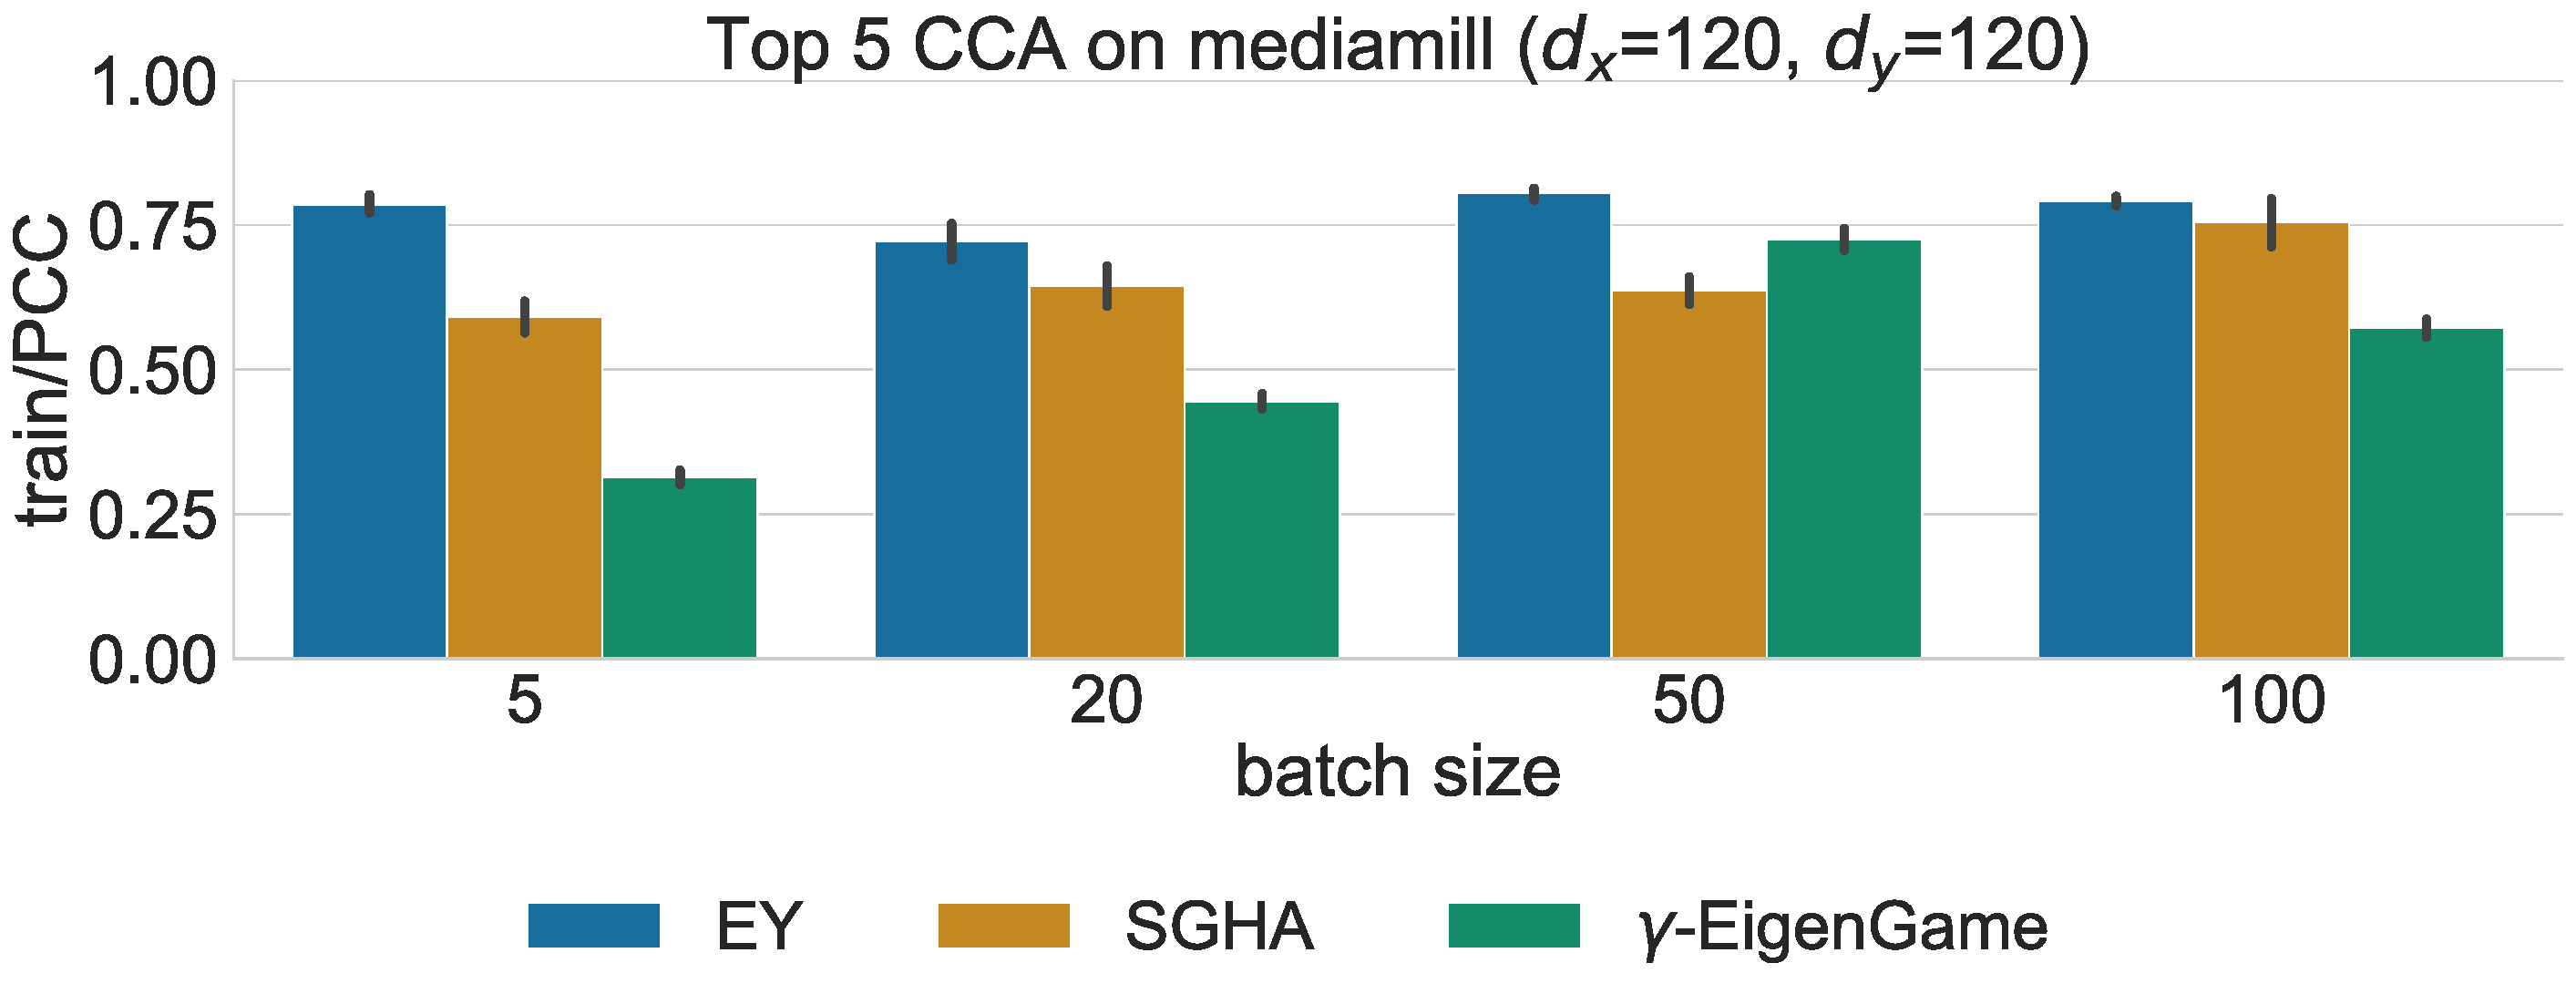
\includegraphics[width=\textwidth]{figures/CCA/mediamill_models_different_batch_sizes}
        \caption{}
        \label{fig:corr_mediamill}
    \end{subfigure}
    \hfill
    \begin{subfigure}[b]{0.49\textwidth}
        \centering
        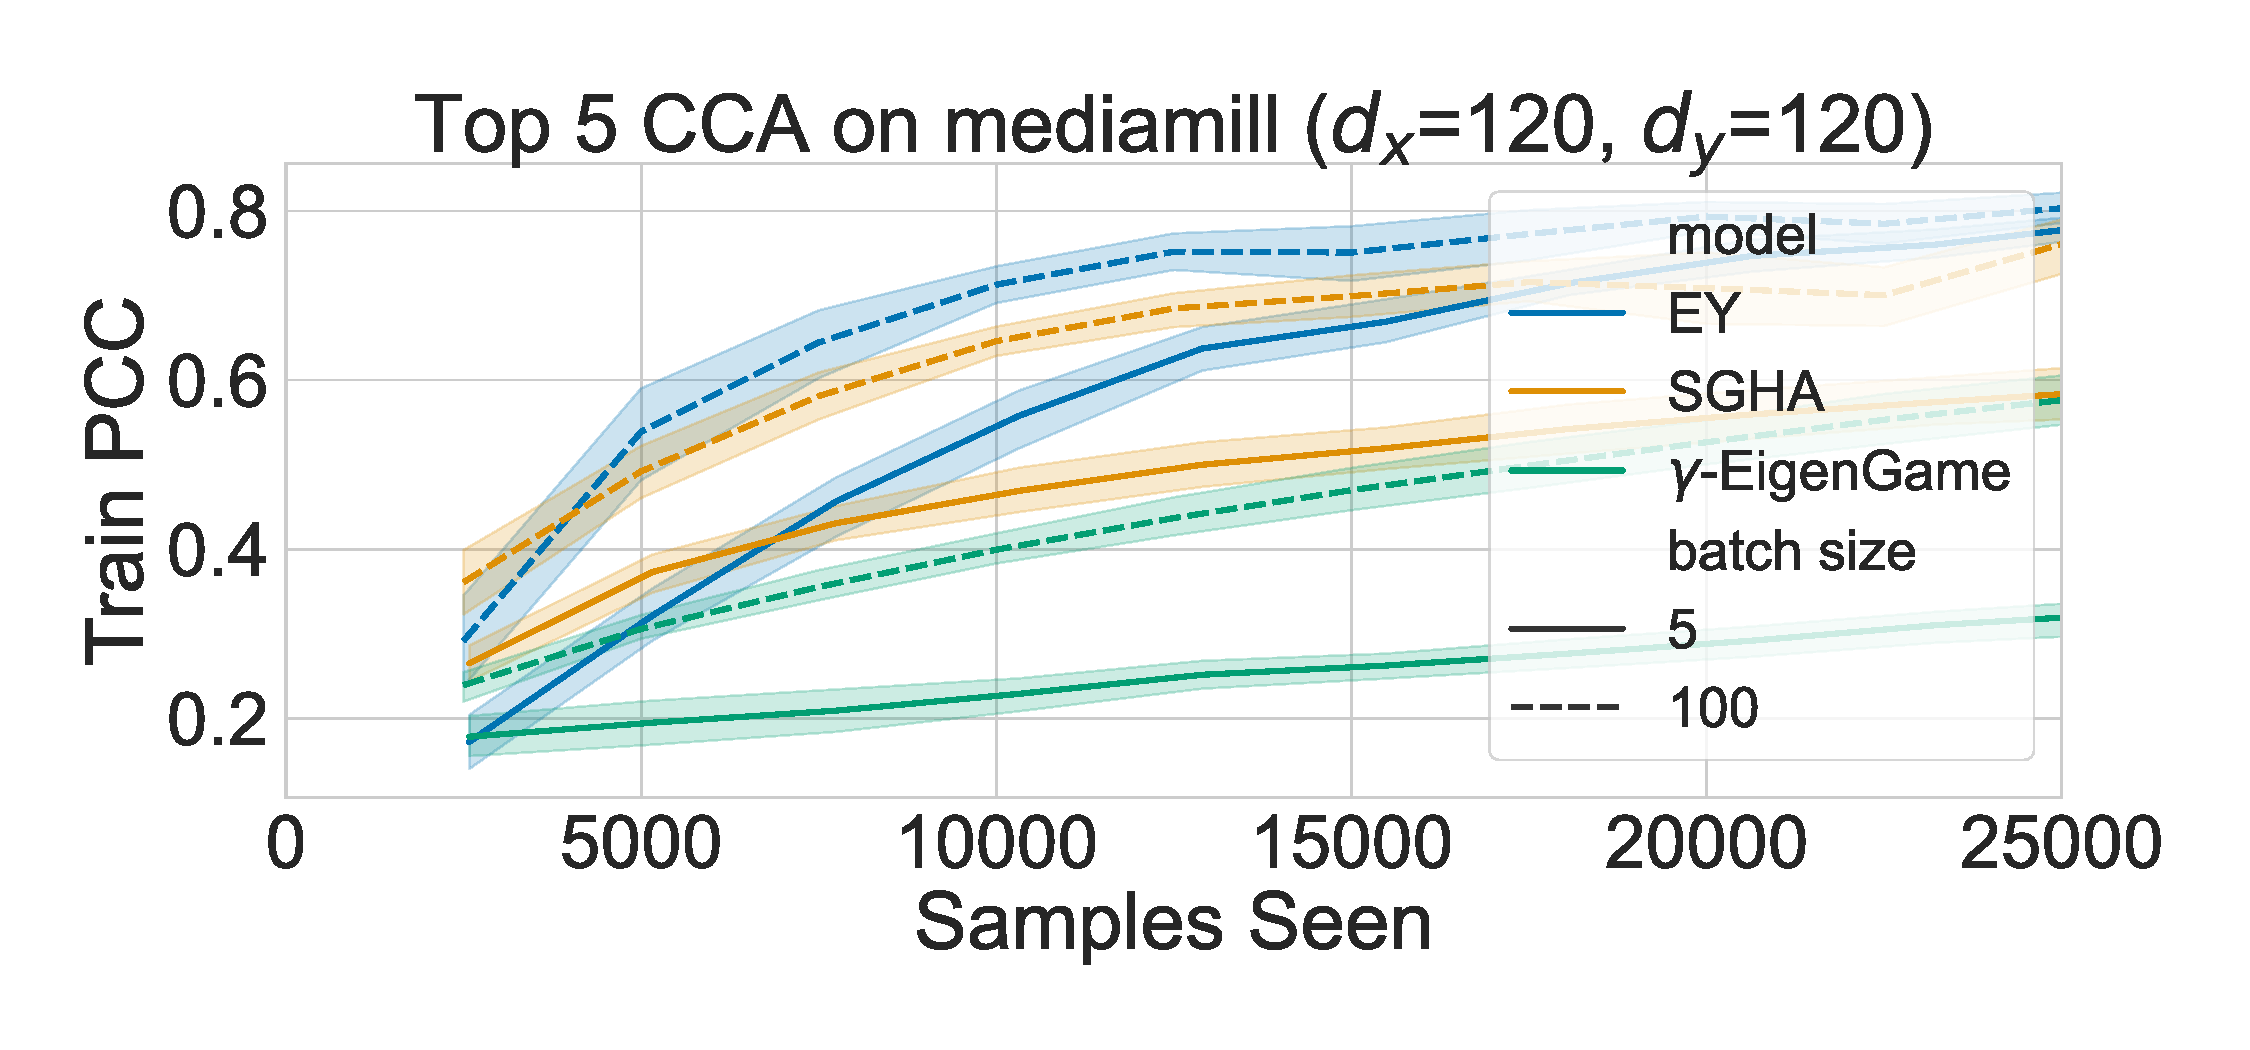
\includegraphics[width=\textwidth]{figures/CCA/mediamill_allbatchsizes_pcc}
        \caption{}
        \label{fig:lr_mediamill}
    \end{subfigure}
    \caption{Stochastic CCA on MediaMill using the Proportion of Correlation Captured (PCC) metric: (a) Across varying mini-batch sizes, trained for a single epoch, and (b) Training progress over a single epoch for mini-batch sizes 5, 100.
    Shaded regions signify \(\pm\) one standard deviation around the mean of 5 runs.}\label{fig:scca_mediamill}
\end{figure}

\begin{figure}
    \centering
    \begin{subfigure}[b]{0.49\textwidth}
        \centering
        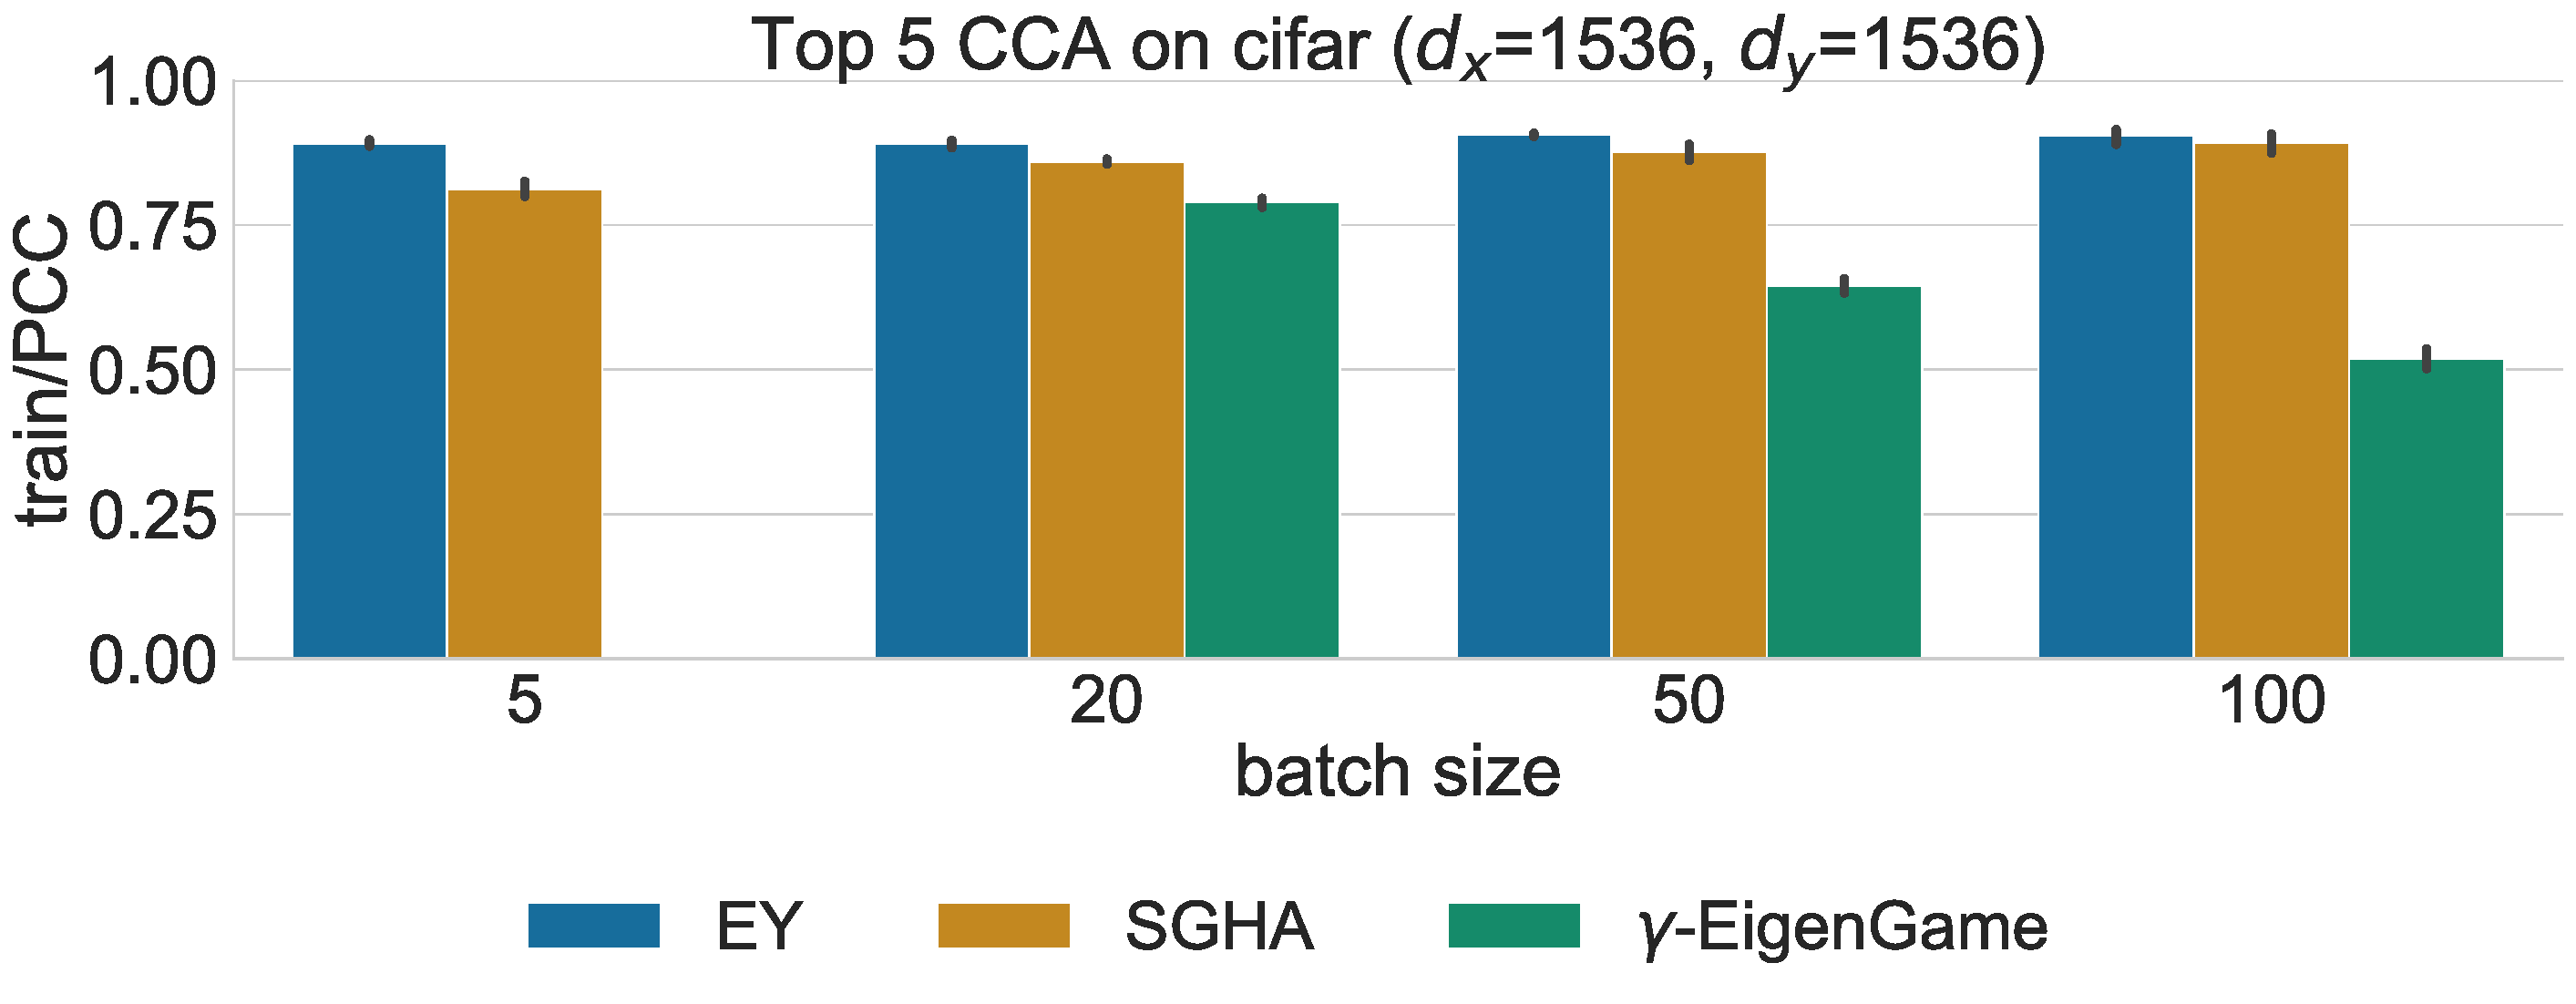
\includegraphics[width=\textwidth]{figures/CCA/cifar_models_different_batch_sizes}
        \caption{}
        \label{fig:corr_cifar}
    \end{subfigure}
    \hfill
    \begin{subfigure}[b]{0.49\textwidth}
        \centering
        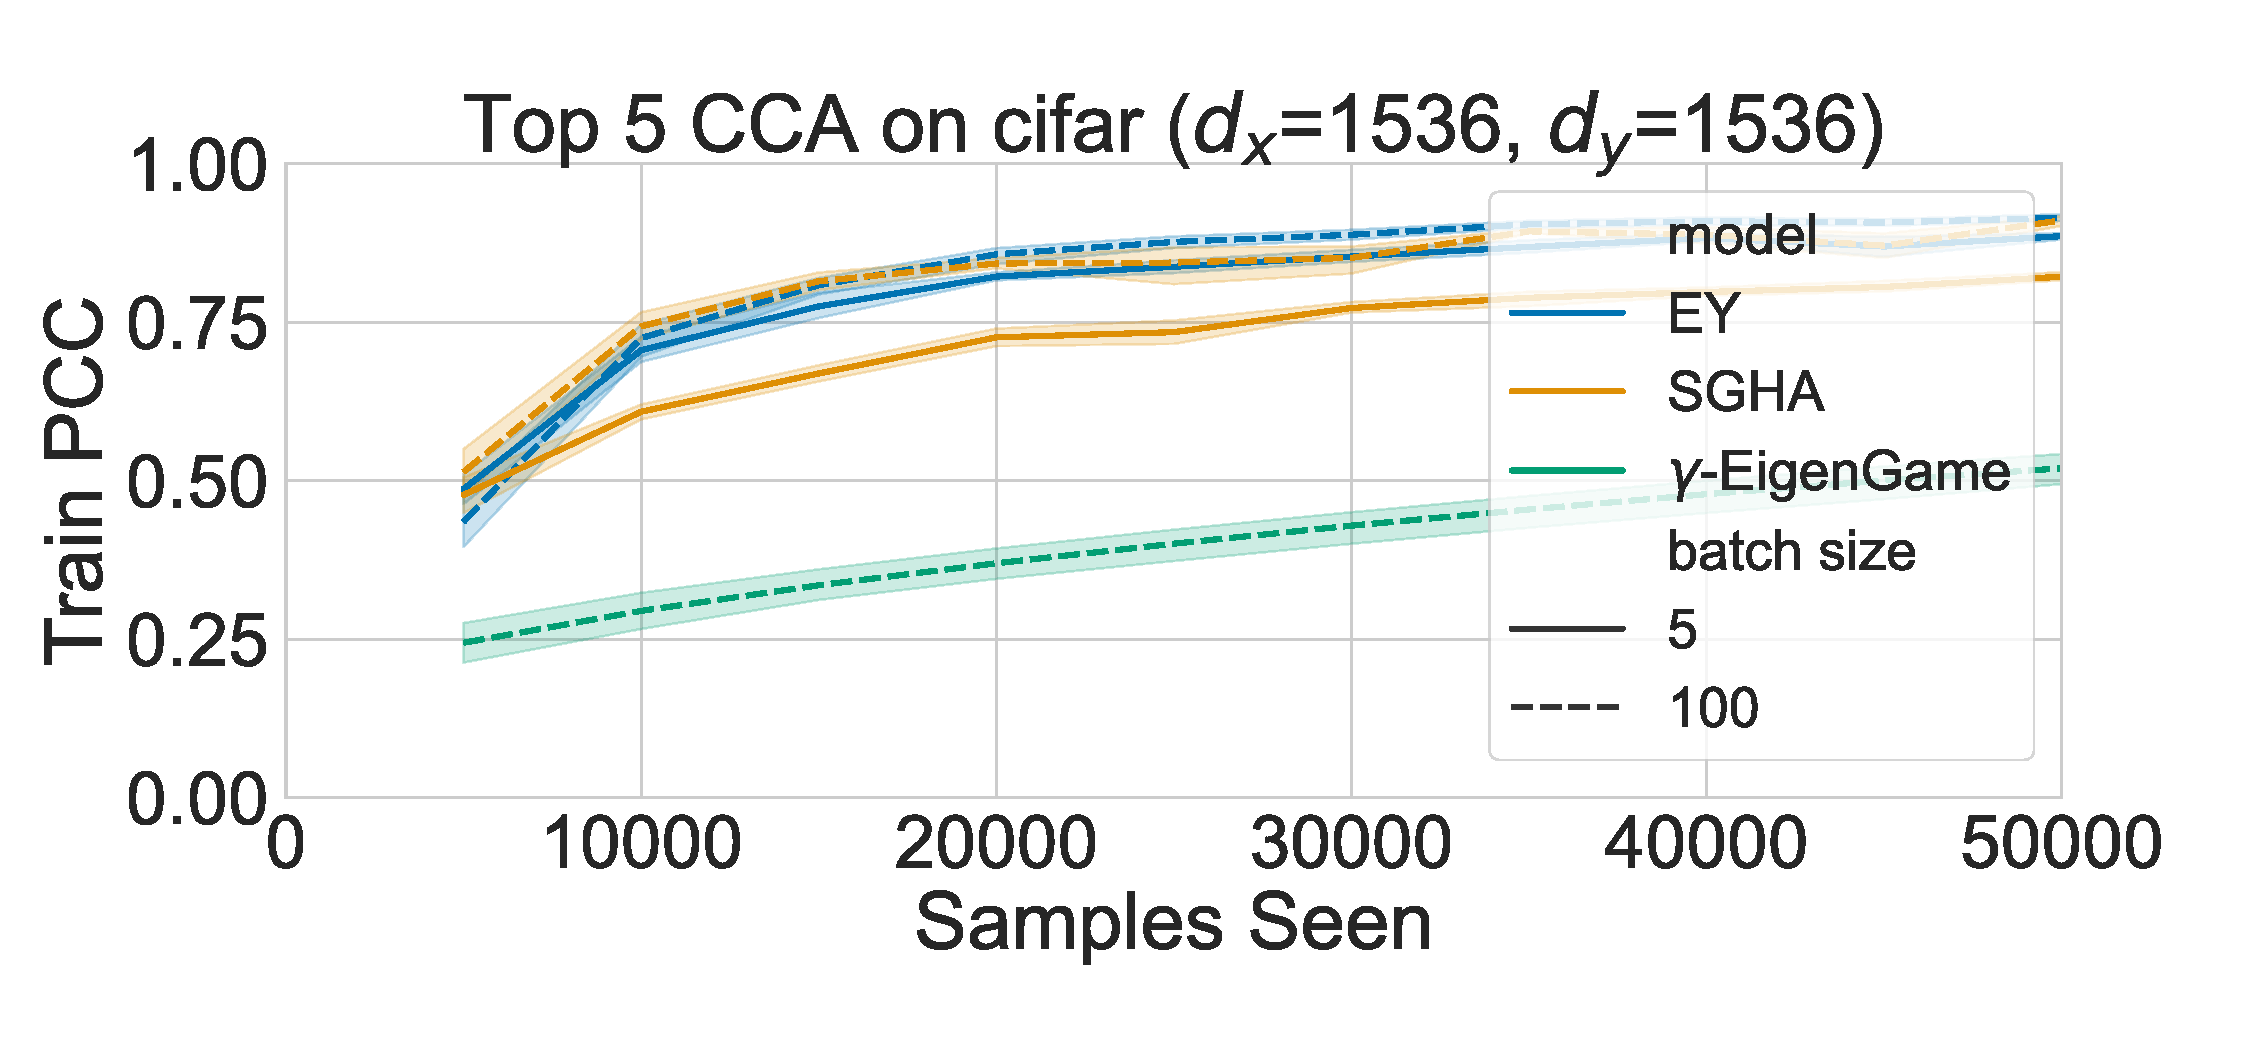
\includegraphics[width=\textwidth]{figures/CCA/cifar_allbatchsizes_pcc}
        \caption{}
        \label{fig:lr_cifar}
    \end{subfigure}
    \caption{Stochastic CCA on CIFAR using the Proportion of Correlation Captured (PCC) metric: (a) Across varying mini-batch sizes, trained for a single epoch, and (b) Training progress over a single epoch for mini-batch sizes 5, 100.
    Shaded regions signify \(\pm\) one standard deviation around the mean of 5 runs.}\label{fig:scca_cifar}
\end{figure}

\subsection{Stochastic PLS UK Biobank}
Next, we demonstrate the scalability of our methods to extremely high-dimensional data by applying stochastic PLS to imaging genetics data from the UK Biobank \citep{sudlow2015uk}.
PLS is typically used for imaging-genetics studies owing to the extremely high dimensionality of genetics data requiring lots of regularisation.
PLS can reveal novel phenotypes of interest and uncover genetic mechanisms of disease and brain morphometry.
Previous imaging genetics analyses using full-batch PLS were limited to much smaller datasets \citep{Lorenzi2018,Taquet2021,Lefloch2012}.
The only other analysis on the UK Biobank at comparable scale partitions the data into clusters and bootstrapping local PLS solutions on these clusters \citep{lorenzi2017secure, altmann2023tackling}.
We ran PLS-EY with mini-batch size 500 on brain imaging (82 regional volumes) and genetics (582,565 variants) data for 33,333 subjects. See supplement (Section \ref{sec:ukbb_preprocessing}) for data pre-processing details.
To our knowledge, this is the largest-scale PLS analysis of biomedical data to-date.

\textbf{Further details:} The UK BioBank data consisted of real-valued continuous brain volumes and ordinal, integer genetic variants.
We used pre-processed (using FreeSurfer \citep{Fischl2012}) grey-matter volumes for 66 cortical (Desikan-Killiany atlas) and 16 subcortical brain regions and 582,565 autosomal genetic variants.
The affects of age, age squared, intracranial volume, sex, and the first 20 genetic principal components for population structure were removed from the brain features using linear regression to account for any confounding effects.
Each brain ROI was normalized by removing the mean and dividing the standard deviation.
We processed the genetics data using PLINK \citep{Purcell2007} keeping genetic variants with a minor allele frequency of at least 1\%  and a maximum missingness rate of 2\%.
We used mean imputation to fill in missing values and centered each variant.

To generate measures of genetic disease risk, we calculated polygenic risk scores using PRSice \citep{PRSice2014}. We calculated scores, with a p-value threshold of 0.05, using GWAS summary statistics for the following diseases; Alzheimer's \citep{Lambert2013}, Schizophrenia \citep{Trubetskoy2022}, Bipolar \citep{Mullins2021}, ADHD \citep{Demontis2023}, ALS \citep{Van_Rheenen2021}, Parkinson's \citep{Nalls2019}, and Epilepsy \citep{International_League_Against_Epilepsy_Consortium_on_Complex_Epilepsies2018}, using the referenced GWAS studies.

The GEP-EY PLS analysis was trained for 100 epochs using a learning rate of 0.0001 with a minibatch size of 500.

\textbf{Observations:} We see strong validation correlation between all 10 corresponding pairs of vectors in the PLS subspace and weak cross correlation, indicating that our model learnt a coherent and orthogonal subspace of covariation (Figure \ref{fig:UKBB_corr}), a remarkable feat for such high-dimensional data. We found that the PLS brain subspace was associated with genetic risk measures for several disorders (Figure \ref{fig:genetic_risk}), suggesting that the PLS subspace encodes relevant information for genetic disease risk, a significant finding for biomedical research.

\begin{figure}
    \centering
    \begin{subfigure}[b]{0.27\textwidth}
        \centering
        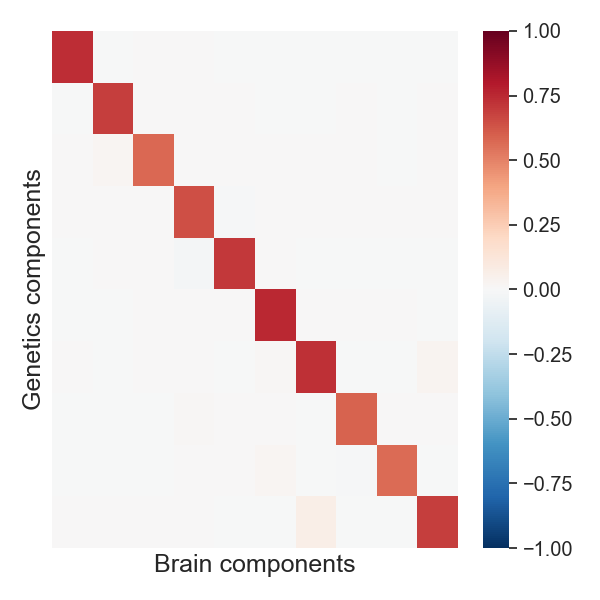
\includegraphics[width=\textwidth,trim={0.8cm 0cm 0.3cm 0cm}]{figures/UKBB/cross_corr.png}
        \caption{}
        \label{fig:UKBB_corr}
    \end{subfigure}
    \begin{subfigure}[b]{0.72\textwidth}
        \centering
        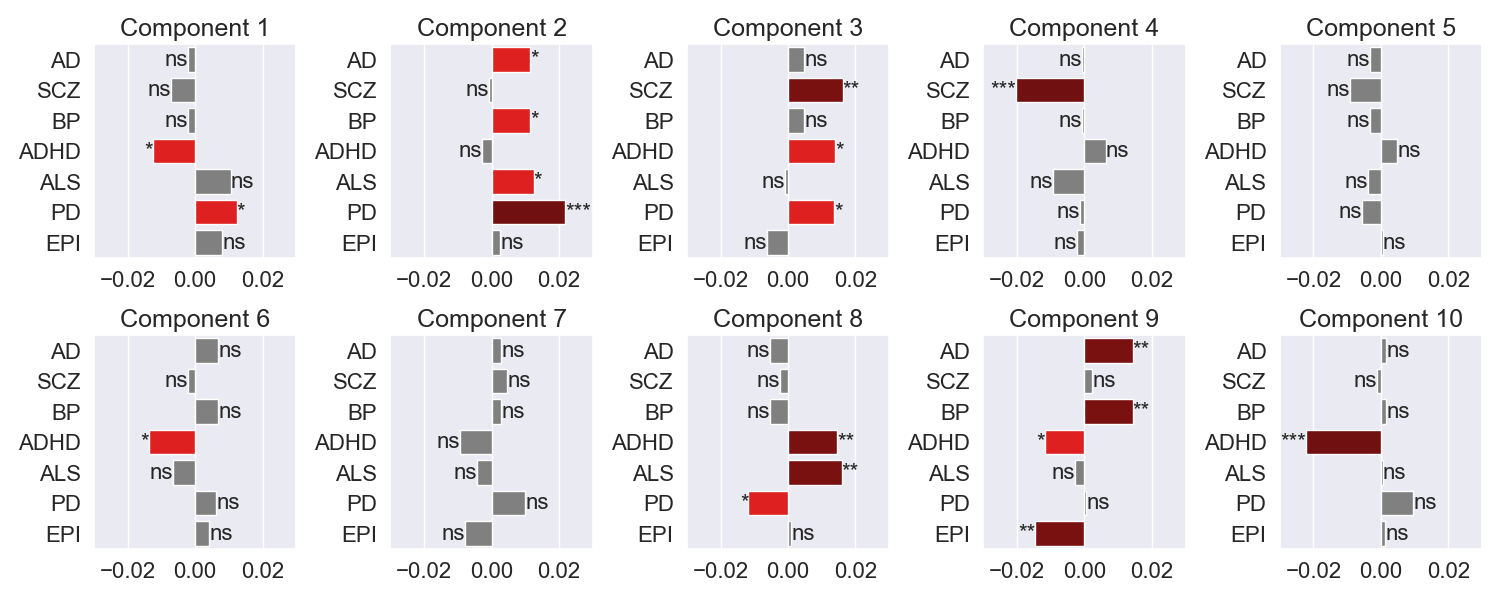
\includegraphics[width=\textwidth,trim={0.5cm 0cm 0.7cm 0cm}]{figures/UKBB/prs_correlations.png}
        \caption{}
        \label{fig:genetic_risk}
    \end{subfigure}
    \caption{(a) Correlations between PLS components for UK Biobank. (b) Correlations between PLS brain components and genetic risk scores. AD=Alzheimer's disease, SCZ=Schizophrenia, BP=Bipolar, ADHD=Attention deficit hyperactivity disorder, ALS=Amyotrophic lateral sclerosis, PD=Parkinson's disease, EPI=Epilepsy. $\text{ns}: 0.05< p <= 1, \ast: 0.01< p <=0.05, \ast\ast: 0.001< p <= 0.01, \ast\ast\ast: 0.0001< p <= 0.001$.}
\end{figure}

\section{Conclusion}

In this paper, we introduced a class of efficient, scalable algorithms for Canonical Correlation Analysis and Self-Supervised Learning, rooted in a novel unconstrained loss function. These algorithms are computationally lightweight, making them uniquely suited for large-scale problems where traditional methods struggle.

We have two distinct avenues for future research. Firstly, we aim to incorporate regularization techniques to improve both generalizability and interpretability, building upon existing sparse methods in CCA \citep{witten2009extensions}. We also intend to investigate the utility of correlation as a metric for measuring the quality of learnt representations. This holds the potential to replace traditional validation methods like classification accuracy, especially in situations where validation labels are not available.

In summary, this paper sets a new benchmark for addressing large-scale CCA problems and opens new avenues in self-supervised learning, paving the way for more accessible and efficient solutions in various applications.